 \documentclass[12pt]{article}
\usepackage{graphicx} % for inserting images
\usepackage[utf8]{inputenc} % for good practice
\usepackage{amsmath} % for equations
\usepackage{amsfonts}
\usepackage{hyperref}
\usepackage[ruled,linesnumbered]{algorithm2e}
\usepackage{setspace}
\usepackage{siunitx}
\sisetup{output-exponent-marker=\ensuremath{\mathrm{e}}}

\newcommand{\norm}[1]{\left\lVert#1\right\rVert}
\newcommand{\abs}[1]{\lvert#1\rvert}

\title{Support Vector Regression\\using\\Deflected Subgradient Methods}
\author{Elia Piccoli\\Nicola Gugole}
\begin{document}
	\begin{titlepage}
		\maketitle
		\pagenumbering{gobble}
	   \begin{center}
		\vspace{0.5cm}
	        \textit{A project presented for the\\Computational Mathematics for Learning and Data Analysis\\course}
	       \vfill	     
	       
\includegraphics[width=0.2\textwidth]{unipi.png}\\
	       University of Pisa\\
	       Artificial Intelligence\\
			A.Y. 2020/2021\\
	            
	   \end{center}
	\end{titlepage}
	
	\newpage
	\tableofcontents
	\vspace{4cm}
	\begin{abstract}
		 Project aim is developing the implementation of a model which follows an SVR-type approach including various different kernels. The implementation uses as optimization algorithm a dual approach with appropriate choices of the constraints to be dualized, where the Lagrangian Dual is solved by an algorithm of the class of deflected subgradient methods.
	\end{abstract}
	\pagenumbering{arabic} %per rimettere i numeri di pagina
	\pagebreak
	\section{Introduction}
Per affrontare questo problema di regressione ci vogliamo affidare ad un modello di apprendimento supervisionato che è il Support Vector Regression. SVR ha come obiettivo trovare una funzione tale per cui ogni record assegnatoci per il training non devii da essa più di  $\varepsilon$  (per questo ogni valore all’interno del cosiddetto $\varepsilon$-tube non viene considerato come errore nella fase di ottimizzazione, rendendo la loss del modello $\varepsilon$-insensitive). Per fare ciò abbiamo bisogno di un certo parametro C (per capire il livello di regolarizzazione che desideriamo) ed un valore $\varepsilon$ (per esprimere l’errore che accettiamo), oltre ad eventuali parametri necessari ad attuare i kernel (e.g. gamma per quanto riguarda il kernel RBF). Parte fondante del modello, oltre a ciò sopra descritto riguardo l’ $\varepsilon$-tube, è dare allo stesso tempo importanza al mantenere la funzione \textit{as flat as possible}, per evitare overfitting ed avere dunque un modello che sia un corretto tradeoff tra accuratezza e generalità.
	\begin{figure}[h]
		\centering
		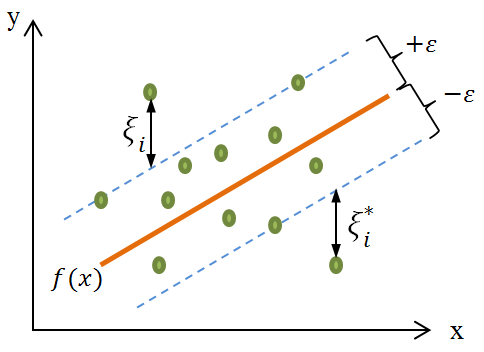
\includegraphics[width=0.5\textwidth]{svrIntro}
		\caption{a generic svr}
		\label{fig:svr_intro}
	\end{figure}

La funzione risultante dall’ottimizzazione del modello è descritta genericamente come:

	\begin{equation}\label{eq:0}
		f(x) = w  x + b
	\end{equation}

Obiettivo dell’ottimizzazione è dunque fare in modo che la curva sia, di nuovo, \textit{as flat as possible}, ma questo è equivalente ad un problema di ottimizzazione dove vogliamo avere $\norm{w}$ minima. 
Per comodità di formulazione del problema possiamo minimizzare $\norm{w}^2$ senza cambiare il significato. Questo ci permette di portarci in un problema di ottimizzazione quadratico, grazie al quale potremo approfittare del concetto di \textbf{strong duality} più tardi. 
Introduciamo a questo punto delle variabili dette \textit{slack} per formulare la \textit{dual objective function}, la quale rappresenta il nostro \textit{primal problem}:
	\begin{equation}\label{eq:1}
		\min_{w,b,\xi_i,\xi_i^*} \frac{1}{2}\norm{w}^2+C\sum_{i}(\xi_{i} + \xi_{i}^*)
	\end{equation}
	Ciò che viene sommato a $\norm{w}$ è un elemento che ci permette di regolare l’errore, e di conseguenza la penalità, dovuti alla possibile presenza di elementi che non rimangono all’interno dell’ $\varepsilon$-tube. Vediamo dunque come C funga da regolarizzatore in una metodica simile a L1. I vari $\xi$ vengono detti \textit{slack variables} e ci permettono di definire i vincoli del problema per qualsiasi i-esimo dato:

	\begin{equation}\label{eq:2}
	\begin{aligned}
		&y_i - w^T\phi(x_i) - b \leq \epsilon + \xi_i,  \\ 
		&b + w^T\phi(x_i) - y_i \leq \epsilon + \xi_i, \\
		&\xi_i,\xi_i^*  \geq 0
	\end{aligned}
	\end{equation}

	\begin{center}
		\footnotesize{$x_i$ input, $y_i$ output}
	\end{center}
	
	Essendo in un problema di ottimizzazione quadratico, la soluzione al \textit{dual problem} risulta equivalente a quella del \textit{primal problem}. In particolare in questa casistica risulta più facile la risoluzione del \textit{dual problem} vista la possibile applicazione del concetto di kernel. Costruiamo dunque il \textit{dual problem} definendo la relativa Lagrangiana (equivalente del \textit{primal problem} al quale aggiungiamo i vincoli sommandoli o sottraendoli):
	

	\begin{equation}\label{eq:3}
	\begin{aligned}
		L(\alpha,\alpha^*,\mu,\mu^*) =  \ &\frac{1}{2}\norm{w}^2\\
		&+C\sum_{i=1}^{m}(\xi_{i} + \xi_{i}^*) \\
		&+ \sum_{i=1}^{m}(\alpha_i(y_i - w^T\phi(x_i) - b - \epsilon - \xi_i))\\
		&+ \sum_{i=1}^{m}(\alpha_i^*(w^T\phi(x_i) + b - y_i - \epsilon - \xi_i^*)) \\
		&- \sum_{i=1}^{m}(\mu_i\xi_i + \mu_i^*\xi_i^*)
	\end{aligned}
	\end{equation}

	A causa del concetto di \textbf{\textit{weak duality}} qualsiasi valore del \textit{primal problem} risulta maggiore (o uguale) del \textit{dual problem}. Da questa considerazione deriviamo il fatto che il punto di massima vicinanza tra i due problemi è dove il \textit{primal problem} ha minimo e il \textit{dual problem} ha massimo. Nella casistica di \textit{strong duality} questa vicinanza si tramuta in uguaglianza.
Cerchiamo dunque di rielaborare il \textit{dual problem} per lavorare con meno variabili possibili, in particolare eliminiamo dai calcoli la variabile w, b e le 2 \textit{slack} $\xi$ e $\xi^*$. In che modo? Stiamo cercando un valore ottimo che tra l’altro sarà unico data la casistica quadratica, dunque la derivata parziale relativa ad ognuna di queste variabili va posta a 0. Questo ci porta a poter ridefinire w:

	\begin{equation}\label{eq:4}
		w = \sum_{i=1}^{m}(\alpha_i - \alpha_i^*)\phi(x_i)
	\end{equation}

	Infine tramite sostituzione nella Lagrangiana definita precedentemente arriviamo ad una funzione dipendente solamente da $\alpha$ e $\alpha^*$:

	\begin{equation}\label{eq:5}
	\begin{aligned}
		\max_{\alpha_i,\alpha_i^*} &- \frac{1}{2}\sum_i\sum_j(\alpha_i - \alpha_i^*)(\alpha_j - \alpha_j^*)K(x_i,x_j) \\
		&- \epsilon\sum_i(\alpha_i + \alpha_i^*)\\
		&+ \sum_i y_i(\alpha_i - \alpha_i^*)
	\end{aligned}
	\end{equation}

	Notiamo che le uniche variabili rimaste sono i moltiplicatori lagrangiani $\alpha$ e $\alpha^*$, i quali sono sottoposti ai seguenti vincoli:
	
	\begin{equation}\label{eq:6}
		\begin{aligned}
		&\forall i \: \alpha_i,\alpha_i^* \geq 0 \qquad\qquad &&(KKT condition) \\
		&\forall i \: \alpha_i,\alpha_i^* \in [0,C]  \qquad\qquad &&(from \: deriving \: \eqref{eq:5})\\
		&\forall i \: \sum (\alpha_i - \alpha_i^*) = 0 \qquad\qquad &&(from \: deriving \: \eqref{eq:5})\\
		&\forall i \: \alpha_i \alpha_i^* = 0 \qquad\qquad &&(from \: model \: construction)
		\end{aligned}
	\end{equation}
			
%discorsi vari sui kernel

	Restando ancora su \eqref{eq:5}, approfondiamo l'elemento $K(x_i,x_j)$, ovvero ciò rappresenta il concetto di \textbf{kernel}, sostituendo ciò che sarebbe un prodotto scalare nello spazio necessitato. Rielaboriamo dunque la precedente frase: certi problemi di regressione non possono essere adeguatamente descritti da modelli lineari. Risulta dunque comodo cambiare spazio di visualizzazione, per portarci in un nuovo spazio (con ogni probabilità con più dimensioni rispetto allo spazio originale) dove il problema diventa linearmente affrontabile. Il cambio di base risulta essere incredibilmente dispendioso per il training del modello ed è proprio in questo caso che il kernel diventa il fulcro dell’efficienza di SVC/SVR. Ci permette infatti di eseguire il \textit{dot-product} nello spazio attuale ma avere come risultato il \textit{dot-product} nello spazio richiesto. Ci permette di risparmiare molte computazioni e di poterle riutilizzare salvandoci i valori risultanti in una \textit{kernel matrix} (riutilizzabile ad ogni ciclo di ottimizzazione). Ovviamente non c’è la certezza di aver preso in considerazione il kernel corretto per la casistica, bisognerà dunque svilupparne vari, magari certi funzioneranno meglio di altri (\textit{rbf, sigmoid, etc}).\\
In particolare questa implementazione prevede il possibile utilizzo di diversi kernel:
	\begin{itemize}
		\item linear: $\langle x,x' \rangle$
		\item polynomial: $(\gamma\langle x,x' \rangle + r)^d$
		\item rbf: $\exp(-\frac{\norm{x-x'}^2}{2\sigma^2})$
		\item sigmoid: $\tanh(\gamma\langle x,x' \rangle + r)$
	\end{itemize}

%discorsi parte finale post definizione problema
	Definito il problema possiamo a questo punto cercare il massimo del \textit{dual problem}. La task da noi scelta utilizzerà \textbf{deflected subgradient methods} per raggiungere l’obiettivo. Una volta raggiunto il massimo avremo a nostra disposizione i corretti $\alpha$ e $\alpha^*$ necessari per il calcolo di $w$. 

	Per completare la funzione risolutrice del problema ci basta trovare il parametro $b$. Ricavarlo risulta semplice se prendiamo in considerazione un qualsiasi elemento del nostro insieme di input tale per cui la relativa predizione $y_i$ sia al limite dell’ $\varepsilon$-tube o al di fuori di esso. Proprio quell’insieme di valori sarà infatti l’unico ad avere come vincoli attivi almeno uno tra i vari $\alpha$ e $\alpha^*$, ovvero un $\alpha$ o $\alpha^*$ diversi da 0. Essendo dunque al margine di un vincolo potremo, derivando da \eqref{eq:0} e \eqref{eq:4}:

	\begin{equation}\label{eq:7}
		x_j \  with\  \alpha_j \in(0,C): b = y_j - \sum_i(\alpha_i - \alpha_i^*)K(x_i,x_j)
	\end{equation}

	Una volta trovata la funzione risultante possiamo testare la bontà del modello effettuando \textit{prediction} su un set di test input per poi calcolare la metrica MSE tra output previsto dal modello e output effettivo del set di test input.\\
Questo fatto è particolarmente importante per il confronto tra modelli e dunque per la ricerca dei parametri migliori possibili (\textit{grid search}).

%dscorsi per spiegare brevemente l'algoritmo, subgradient e deflected
	\section{Basic Algorithms Introduction}
	Come richiesto dalla task utilizzeremo un \textit{subgradient method}, il quale viene utilizzato per trattare funzioni che possono anche avere punti di \textit{nondifferenziabilità}. E’ dunque uno dei metodi più semplici e meno esigenti nei confronti di proprietà necessarie per $f$. In particolare si distingue dagli ordinari metodi di gradiente per due aspetti:
	\begin{itemize}
		\item Lo \textit{stepsize} non viene scelto tramite \textit{line search} ma tramite altri ragionamenti (il più immediato tra tutti è \textbf{DSS}, dove lo stepsize viene fissato a priori con degli appropriati vincoli di scelta)
		\item Non è un \textit{descent method}, ovvero il valore della funzione può incrementare nelle iterazioni. Questo avviene per il motivo che non tutti i subgradient portano a direzioni di discesa. Anche se questo è vero abbiamo provato durante il corso che iterazioni successive ci portano ad avvicinarci a $x^*$ monotonicamente scelta una corretta \textit{stepsize}. Con questa certezza sappiamo che convergeremo lentamente ma sicuramente ad $x^*$ e di conseguenza anche ad $f^*$ (anche se probabilmente non monotonicamente).  
	\end{itemize}
	Entrando più nel dettaglio per quanto riguarda lo \textit{stepsize}, la scelta di fissarlo a priori (DSS) ci porta ad una convergenza estremamente lenta, dunque preferiremmo utilizzare altre euristiche. In particolare, se avessimo a disposizione f* potremmo seguire la \textit{Polyak stepsize} (\textbf{PSS}), la quale ci permette di determinare lo stepsize ottimo basandosi sulla seguente formula:
	
	\begin{equation}\label{eq:polyak}
		\alpha_i = \beta_i\frac{f(x_i) - f(x^*)}{\norm{g_i}^2}
	\end{equation}

	Notiamo la necessità di un ulteriore parametro $\beta$, il quale deve rispettare il vincolo $\beta \in [0,2]$.\\
	Purtroppo nel nostro caso non siamo a conoscenza di $f^*$ e dobbiamo di conseguenza introdurre la tecnica che verrà utilizzata in Algorithm\ref{algo:2}, ovvero \textit{Target Level Stepsize}. Essa si basa sullo stimare $f^*$ per poter poi attuare la stessa formulazione di  Polyak, rimanendo sempre pronto a rivalutare la stima nel momento in cui una nuova e migliore stima viene ottenuta.\\
	Più approfonditamente la tecnica Target Value utilizza dei parametri $\rho$ e $\delta$, tramite i quali, dopo aver fissato una stima iniziale $fref$, ci permette di aggiornare la stima secondo i seguenti concetti:
	\begin{itemize}
	\item $\delta$ (parametro che segue il vincolo $\delta > 0$) ci permette di definire una stima di $f^*\longrightarrow fref - \delta$ tale per cui la stima $fref$ verrà aggiornata solo se troveremo un valore $f$ che migliori decisamente la stima (ovvero $f < fref - \delta$).
	\item$\rho$ (parametro che segue il vincolo $\rho \in (0,1)$) ci permette di ottenere un vanishing $\delta$, ovvero dopo aver superato una certa threshold andremo a rimpicciolire $\delta \longrightarrow (\delta = \rho \cdot \delta)$. Questo viene effettuato perché più ci avvicineremo alla soluzione più il range che ci distanzia da $f^*$ rimpicciolisce, lasciando meno spazio di miglioramento ad $f$.
	\end{itemize}
	L’altro elemento richiestoci dalla task è l’utilizzo di un \textit{deflected method}. Questa metodologia ci permette di basare il nuovo punto di valutazione di $f$ (ovvero $x_i$) non solo dando peso al subgradient calcolato ma anche basandosi sulla \textit{precedente direzione intrapresa}, evitando un andamento esageratamente a zig zag. Per pesare le due parti necessitiamo di un parametro $\gamma$ (vincolato tra 0 e 1), arrivando alla formulazione: 
	\begin{equation}\label{eq:direction}
		d_i = \gamma_ig_i + (1 - \gamma_i) d_{i-1}
	\end{equation}
	In particolare all’interno di Algorithm\ref{algo:2} andremo ad utilizzare l’approccio \textit{deflection-first/stepsize-restricted}, ovvero ad ogni iterazione definiremo innanzitutto la direzione $d$ da intraprendere seguendo \eqref{eq:direction} per poi ottenere lo $stepsize$:
	\begin{equation}\label{eq:stepsize}
		stepsize_i = \beta_i\frac{f(x_i) - fref + \delta}{\norm{d_i}^2}
	\end{equation}
	Vincolando $\beta \longrightarrow \beta \leq \gamma$.

	\pagebreak
%discorsi su strutture necessarie per implementazione e motivazioni per scelte
	\section{Structures for implementation}
	Passando dalla formalizzazione matematica vista nella sezione precedente giungiamo alla sua implementazione. In Algorithm\ref{algo:1}, partendo dai dati di input ed il rispettivo output, vengono calcolati i valori dei moltiplicatori lagrangiani i quali successivamente permettono di trovare il valore di $w$ e $b$.
L’obiettivo è quindi quello di rappresentare il problema di massimizzazione formalizzato in \eqref{eq:5}. Per comodità il primo passaggio è trasformare la ricerca di un massimo nella ricerca di un minimo, facilmente attuabile tramite il cambio di segno della nostra funzione. Successivamente vanno definite le matrici e i vincoli che ci permettono di rappresentare il \textit{Quadratic Problem}:\\
	\begin{equation}\label{eq:8}
		\min \frac{1}{2}x'Qx + qx \longrightarrow \forall_i\; lower\_bound\leq x_i\leq upper\_bound
	\end{equation}

	Analizziamo quindi la formalizzazione dei singoli componenti di \eqref{eq:8} insieme ad altri componenti necessari all'implementazione:
	
	\begin{itemize}
		\item \textbf{kernel matrix}: presi $m$ record di input sarà una matrice simmetrica $ K(x,x') \in \mathbb{R}^{m,m}$
		\item \textbf{alpha matrix ($x$)}: presi $m$ record di input sarà un vettore $ x \in \mathbb{R}^{2m} $ tale per cui $x_i \neq 0$ solo se il relativo input genera un output che contribuisce alla $loss$ . Prima metà di $x$ rappresenterà l'insieme di $\alpha$ mentre la seconda metà rappresenterà l'insieme di $\alpha*$ .
		\item \textbf{Q}: da \eqref{eq:5} si nota che è rappresentato dalla \textit{kernel matrix}, fatto non sufficiente per assicurare la proprietà di essere \textit{positive semi-definite}, abbreviato da qui in poi con \textbf{PSD} (basta pensare al kernel \textit{sigmoid}). La formalizzazione che viene utilizzata all’interno di Algorithm\ref{algo:1} \linebreak{[ \ref{bib:1} ]} ci assicura invece la proprietà di \textbf{PSD},  lo spazio del problema diventa dunque convesso assicurandoci che punti stazionari sono anche di minimo globale, proprietà non ottenuta da altri modelli (per esempio NN). 
		\item \textbf{q}: costruita in modo da unire i rimanenti elementi di \eqref{eq:5}.
		\item \textbf{linear constraint}: il vincolo lineare presente sui moltiplicatori lagrangiani ci permette di definire $lb=0$ e $ub=C$.
	\end{itemize}
		
	Data questa formalizzazione tramite Algorithm\ref{algo:2} verrà risolto il problema di minimizzazione ottenendo i valori dei moltiplicatori lagrangiani. A questo punto sarà quindi possibile calcolare il valore di $w$ e $b$ in modo tale da rappresentare la nostra funzione:
	\begin{center}
		$f(x)=wx+b$
	\end{center}

	In particolare, per determinare il valore di $b$ andremo ad applicare quanto già evidenziato precedentemente in \eqref{eq:7}, sarà necessario trovare un elemento che si trovi al di fuori dell’$\varepsilon$-tube e rispetto quest’ultimo calcolare il valore.


%pseudocodice e analisi parti importanti
	\section{Pseudo Code}
	\begin{algorithm}[H]
		\scriptsize
		\DontPrintSemicolon
		\label{algo:1}
		\KwIn{$X$ input matrix of size $m \times d$ \newline
			$y$  output vector of size $m$\newline
			$C$ regularization parameter\newline
			$\varepsilon$  parameter defining sensitiveness of model\newline
			$kernel\_type$ defining which kernel to use\newline
			$args$ necessary and different for each kernel}
		\KwOut{Parameters $w$ e $b$ for resulting function ( $ f(x) = wx + b $ )}
		\setstretch{1.1}
		
		\Begin{
			$K \longleftarrow kernel(X, kernel\_type, args)$\\
			\tcp{to assure $Q$ to be Positive Semidefinite}
			$Q \longleftarrow [K\qquad -K ;\qquad -K \qquad\;  K]$\\
			$q \longleftarrow [-y\qquad y]$\\
			$q \longleftarrow q + \varepsilon$\\
			$upper\_bound \longleftarrow C$\\
			$alphas \longleftarrow Fit\_SVR(Q,q,upper\_bound)$\\
			$alpha^+ \longleftarrow alphas_{0:(size(alphas)/2)}$\\
			$alpha^- \longleftarrow alphas_{(size(alphas)/2):size(alphas)}$\\
			$w \longleftarrow (alpha^+ - alpha^-)K$\\
			\tcp{first $i \;|\; alpha_i^+ \ne 0 $ or $alpha_i^- \ne 0$  $\longrightarrow alpha\_not\_zero = i$}
			$b = y_{alpha\_not\_zero} - \sum_i (alpha^+_i - alpha^-_i)K_{i,alpha\_not\_zero}$\\
		}
		 \caption{Get\_SVR}
	\end{algorithm}
	\pagebreak
	\begin{algorithm}[H]
		\scriptsize
		\DontPrintSemicolon
		\label{algo:2}
		\KwIn{$Q$ input matrix of size $2m \times 2m$ \newline
		$q$  output vector of size $2m$\newline
		$ub$ upper bound for constrained variables\newline
		$stopping\_criterion$ $(default = \num{1e-12})$\newline
		$\gamma$ for Deflection $(default = 0.5)$\newline
		$\beta$ for Target Level $(default = 0.5)$\newline
		$eps$ for Target Level $(default = \num{1e-6})$\newline
		$\delta\_reset$ for Target Level $(default = \num{1e-4})$\newline
		$\rho$ for Target Level $(default = 0.95)$\newline
		$maxiter$ for stopping iteration $(default = 1000)$
		}
			
		\KwOut{Optimal $x$ to minimize constrained $\frac{1}{2}x'Qx + qx$}
		\setstretch{1.1}
		
		\Begin{
		$x \longleftarrow ([0] \cdot size(q))'$ \hfill \texttt{// init of lagrangian multipliers}\\
		$xref \longleftarrow x$\\
		$fref \longleftarrow inf$\\
		$\delta \longleftarrow 0$\\
		$dprev \longleftarrow 0$\\
		$iter \longleftarrow 1$\\
		\While{true}{
			\texttt{// check if in $stopped$ condition}\\
			\If{$iter > maxiter$}{
				return $xref$\\
				}

			$v \longleftarrow \frac{1}{2}x'Qx + qx$\\
			$g \longleftarrow Qx + q$\\
			\texttt{// check if in $optimal$ condition}\\
			\If{$\norm{g} < stopping\_criterion$}{
				return $x$\\
				}
			
			\texttt{// reset $\delta$ if $v$ is \textit{good} or decrease it otherwise}\\
			\eIf{$v \leq fref - \delta$}{
				$\delta \longleftarrow \delta\_reset \cdot \max{v,1}$\\
				}{
				$\delta \longleftarrow \max(\delta \rho , eps \cdot\max(\abs{ \min(v,fref) } , 1) )$\\
				}
			\texttt{// update $fref$ and $xref$ if needed}\\
			\If{$v < fref$}{
				$fref \longleftarrow v$\\
				$xref \longleftarrow x$\\
				}
			\texttt{// compute $stepsize$ and new $x$}\\
			$d,dprev \longleftarrow$ Get\_Direction$(\gamma,g,dprev,ub,x)$\\
			$stepsize \longleftarrow \frac{\beta(v-fref+\delta)}{\norm{d}^2}$ \hfill \texttt{// deflection-first $\rightarrow \beta \leq \gamma$}\\
			$x \longleftarrow x - stepsize\cdot d$\\
			$iter \longleftarrow iter + 1$\\
			}
		}
		 \caption{Fit\_SVR}
	\end{algorithm}

	\newpage

	\begin{algorithm}[H]
		\DontPrintSemicolon
		\scriptsize
		\KwIn{$\gamma \in [0,1]$ needed for Deflection $(default = 0.5)$\newline
				$g$ gradient\newline
				$dprev$ previous direction for Deflection\newline
				$ub$ upperbound for ensuring constraints\newline
				$x$ constrained variable $\longrightarrow x \in [0,ub]$\newline
		}
			
		\KwOut{$d$ direction for next step\newline$dprev$ updated previous direction\newline}
		\setstretch{1.1}
		
		\Begin{
			\texttt{// compute direction $d$ using deflection}\\
			$d \longleftarrow \gamma g + (1 - \gamma)dprev$\\
			\texttt{// ensure constraints $\longrightarrow \forall_i \; x_i \in [0,ub]$}\\
			\For{$i\gets0$ \KwTo $size(x)$}{
    				\If{$(ub-x_i < \num{1e-10} $ and $ d_i < 0)$ or $(x_i < \num{1e-10}$ and $d_i >0)$}{
					$d_i \longleftarrow 0$\\
					}
    				}
			return $d, d$\\
		}
		 \caption{Get\_Direction}
	\end{algorithm}
	\pagebreak
	\section{Doubts}
	\begin{enumerate}
		\item Abbiamo letto diversi paper in letteratura e abbiamo trovato diversi modi in cui viene determinato il valore $b$. Alcuni dicono che basta usare un punto che sia fuori o al margine dell’$\varepsilon$-tube {[ \ref{bib:2} ]}, altri invece lo calcolano su tutti i punti per poi fare una media. C’è un metodo più corretto di un altro? 
		\item Nel calcolo del \textit{Polyak stepsize} utilizziamo un parametro $\beta$ che nel caso di \textit{deflection-first}$ \longrightarrow \beta \leq \gamma$. Nelle slide e appunti però non abbiamo visto nessuna formula rispetto la quale è definito, esiste o è determinato tramite una $grid search$?
		\item Abbiamo visto studiando dagli appunti presi a lezione e dalle slide che $\gamma$ (parametro necessario al \textit{deflected subgradient}) viene definito:\begin{center} $ \gamma_i \in \min\{\norm{\gamma g_i + (1-\gamma)d_{i-1}}^2 : \gamma \in [0,1]\}$\end{center}
		Come ha detto Lei non è obbligatorio avere un valore variabile di $\gamma$ che si adatta a quello che è il comportamento della nostra ricerca del minimo, anche se avere un valore adattivo ci permetterebbe di ottenere risultati migliori. Dobbiamo quindi analizzare entrambe le possibilità? Nel caso in cui dovessimo ottenere $\gamma$ tramite minimizzazione dovremo andare a risolvere un problema di minimizzazione ad ogni iterazione del nostro Algorithm\ref{algo:2}? Non diventa \textbf{pesante} dal punto di vista della computazione?
	\end{enumerate}

%riferimenti a documenti citati
	\section{References}
	\begin{enumerate}
		\item \href{https://www.csie.ntu.edu.tw/~cjlin/papers/libsvm.pdf}{LIBSVM: A Library for Support Vector Machines } \label{bib:1}
		\item \href{https://www.cse.iitb.ac.in/~cs709/notes/enotes/svr-kkt-dual-derivation.pdf}{SVR KKT Dual Derivation } \label{bib:2}
	\end{enumerate}
\end{document}